% !TEX root = top.tex
\section{Appendix}
\subsection{Search space}
\paragraph{Standard image classification on CIFAR-10 and ImageNet}
The search space for CIFAR-10 and ImageNet classification experiments includes the following operations:
\begin{itemize}
\item identity
\item $1\times1$ convolution
\item $3\times3$ separable convolution
\item $5\times5$ separable convolution
\item $3\times3$ dilated separable convolution
\item $5\times5$ dilated separable convolution
\item $1\times7$ convolution followed $7\times1$ convolution
\item $3\times3$ max pooling
\item $3\times3$ average pooling
\end{itemize}
A block forms an output by concatenating all leaf nodes in the graph. Blocks have 2 input nodes which ingest the output of block $i-1$ and block $i-2$ respectively. The input nodes are bottleneck layers, and can reduce the spatial size by using stride 2. 

\paragraph{Anytime prediction on CIFAR-10}
The search space for the CIFAR-10 anytime prediction experiments includes the following operations:
\begin{itemize}
\item $1\times1$ convolution
\item $3\times3$  convolution
\item $5\times5$  convolution
\item $3\times3$ max pooling
\item $3\times3$ average pooling
\end{itemize}
In the anytime setting, nodes concatenate their inputs rather than sum. Thus, the identity operator was removed as it would be redundant. The search space does not include separable convolutions so that it is comparable with our baselines \citep{huang2017multi}. Block 1 contains nodes which may operate on any of the 3 scales ($32\times32, 16\times16, 8\times8$). Block 2 contains nodes which can only operate on scales $16\times16$ and $8\times 8$. Block 3 only contains nodes which operate on the scale $8\times 8$. We fix the number of exit nodes. These choices are inspired by  \cite{huang2017multi}

\subsection{Graph HyperNetwork details} 
\paragraph{Standard image classification on CIFAR-10 and ImageNet}
While node embeddings are initialized to a one-hot vector representing computational operator of the node, we found it helpful to pass the sparse vector through a learned embedding matrix  prior to graph propagation. The GHN is trained for 200 epochs  with batch size 64 using the ADAM optimizer with an initial learning rate 1e-3 that is divided by 2 at epoch 100 and 150. A naive hypernet would have a separate output branch for each possible node type, and simply ignore branches that aren't applicable to the specific node. In this manner, the number of parameters of the hypernetwork scale according to the number of possible node computations. In contrast, the number of parameters for a one-shot model scale according to the number of nodes in the graph. We further reduce number of parameters by obtaining smaller sized convolutions kernels through the slicing of larger sized kernels. 

\paragraph{Anytime prediction }
In the anytime prediction setting, two one-hot vectors representing the node's scale and presence of an early exit classifier are additionally concatenated to the first initialized node embedding. We found it helpful to train the GHN with a random number of nodes per block, with maximum number of allowed nodes being the evaluation block size. Because nodes concatenate their inputs, a bottleneck layer is required. The hypernetwork can predict bottleneck parameters for a varying number of input nodes by generating weights based on edge activations rather than node activations. We form edge activations by concatenating the node activations of the parent and child. Edge weights generated this way can be concatenated, allowing the dimensionality of the predicted bottleneck weights the be proportional to the number of incoming edges. 

\subsection{Final architecture training details} 
\paragraph{CIFAR-10} Following existing NAS methods \citep{zoph2017learning,real2018regularized}, the final candidates are trained for 600 epochs  using  SGD with momentum 0.9,  a single period cosine schedule with $l_{max}=0.025$, and batch size 64. For regularization, we use scheduled drop-path with a final dropout probability of 0.4. We use an auxiliary head located at 2/3 of the network weighted by 0.5. We accelerate training by performing distributed training across 32 GPUs; the learning rate is multiplied by 32 with an initial linear warmup of 5 epochs. 

\paragraph{ImageNet Mobile} For ImageNet mobile experiments, we use an image size of $224\times224$. Following existing NAS methods \citep{zoph2017learning,real2018regularized}, the final candidates are trained for 250 epochs using SGD with momentum 0.9, initial learning rate 0.1 multiplied by 0.97 every epoch. We use an auxiliary head located at 2/3 of the network weighted by 0.5. We use the same regularization techniques, and similarly accelerate training in a distributed fashion. 

\paragraph{Anytime}Following \cite{huang2017multi}, the final candidates are trained using SGD with momentum 0.9. We train the models for 300 epochs use an initial learning rate of 0.1, which is divided by 10 after 150 and 225 epochs using a batch size of 64. We accelerate training with distributed training in a similar fashion as the CIFAR-10 classification and ImageNet mobile experiments. 
The number of filters for the final architecture is chosen such that the number of FLOPS is comparable to existing baselines.


\subsection{Visualization of Final architectures}
\subsubsection{CIFAR-10 and ImageNet Classification}
Figure \ref{fig:best_block} shows the best found block in the CIFAR-10 Experiments.

\begin{figure}[h]
\iflatexml
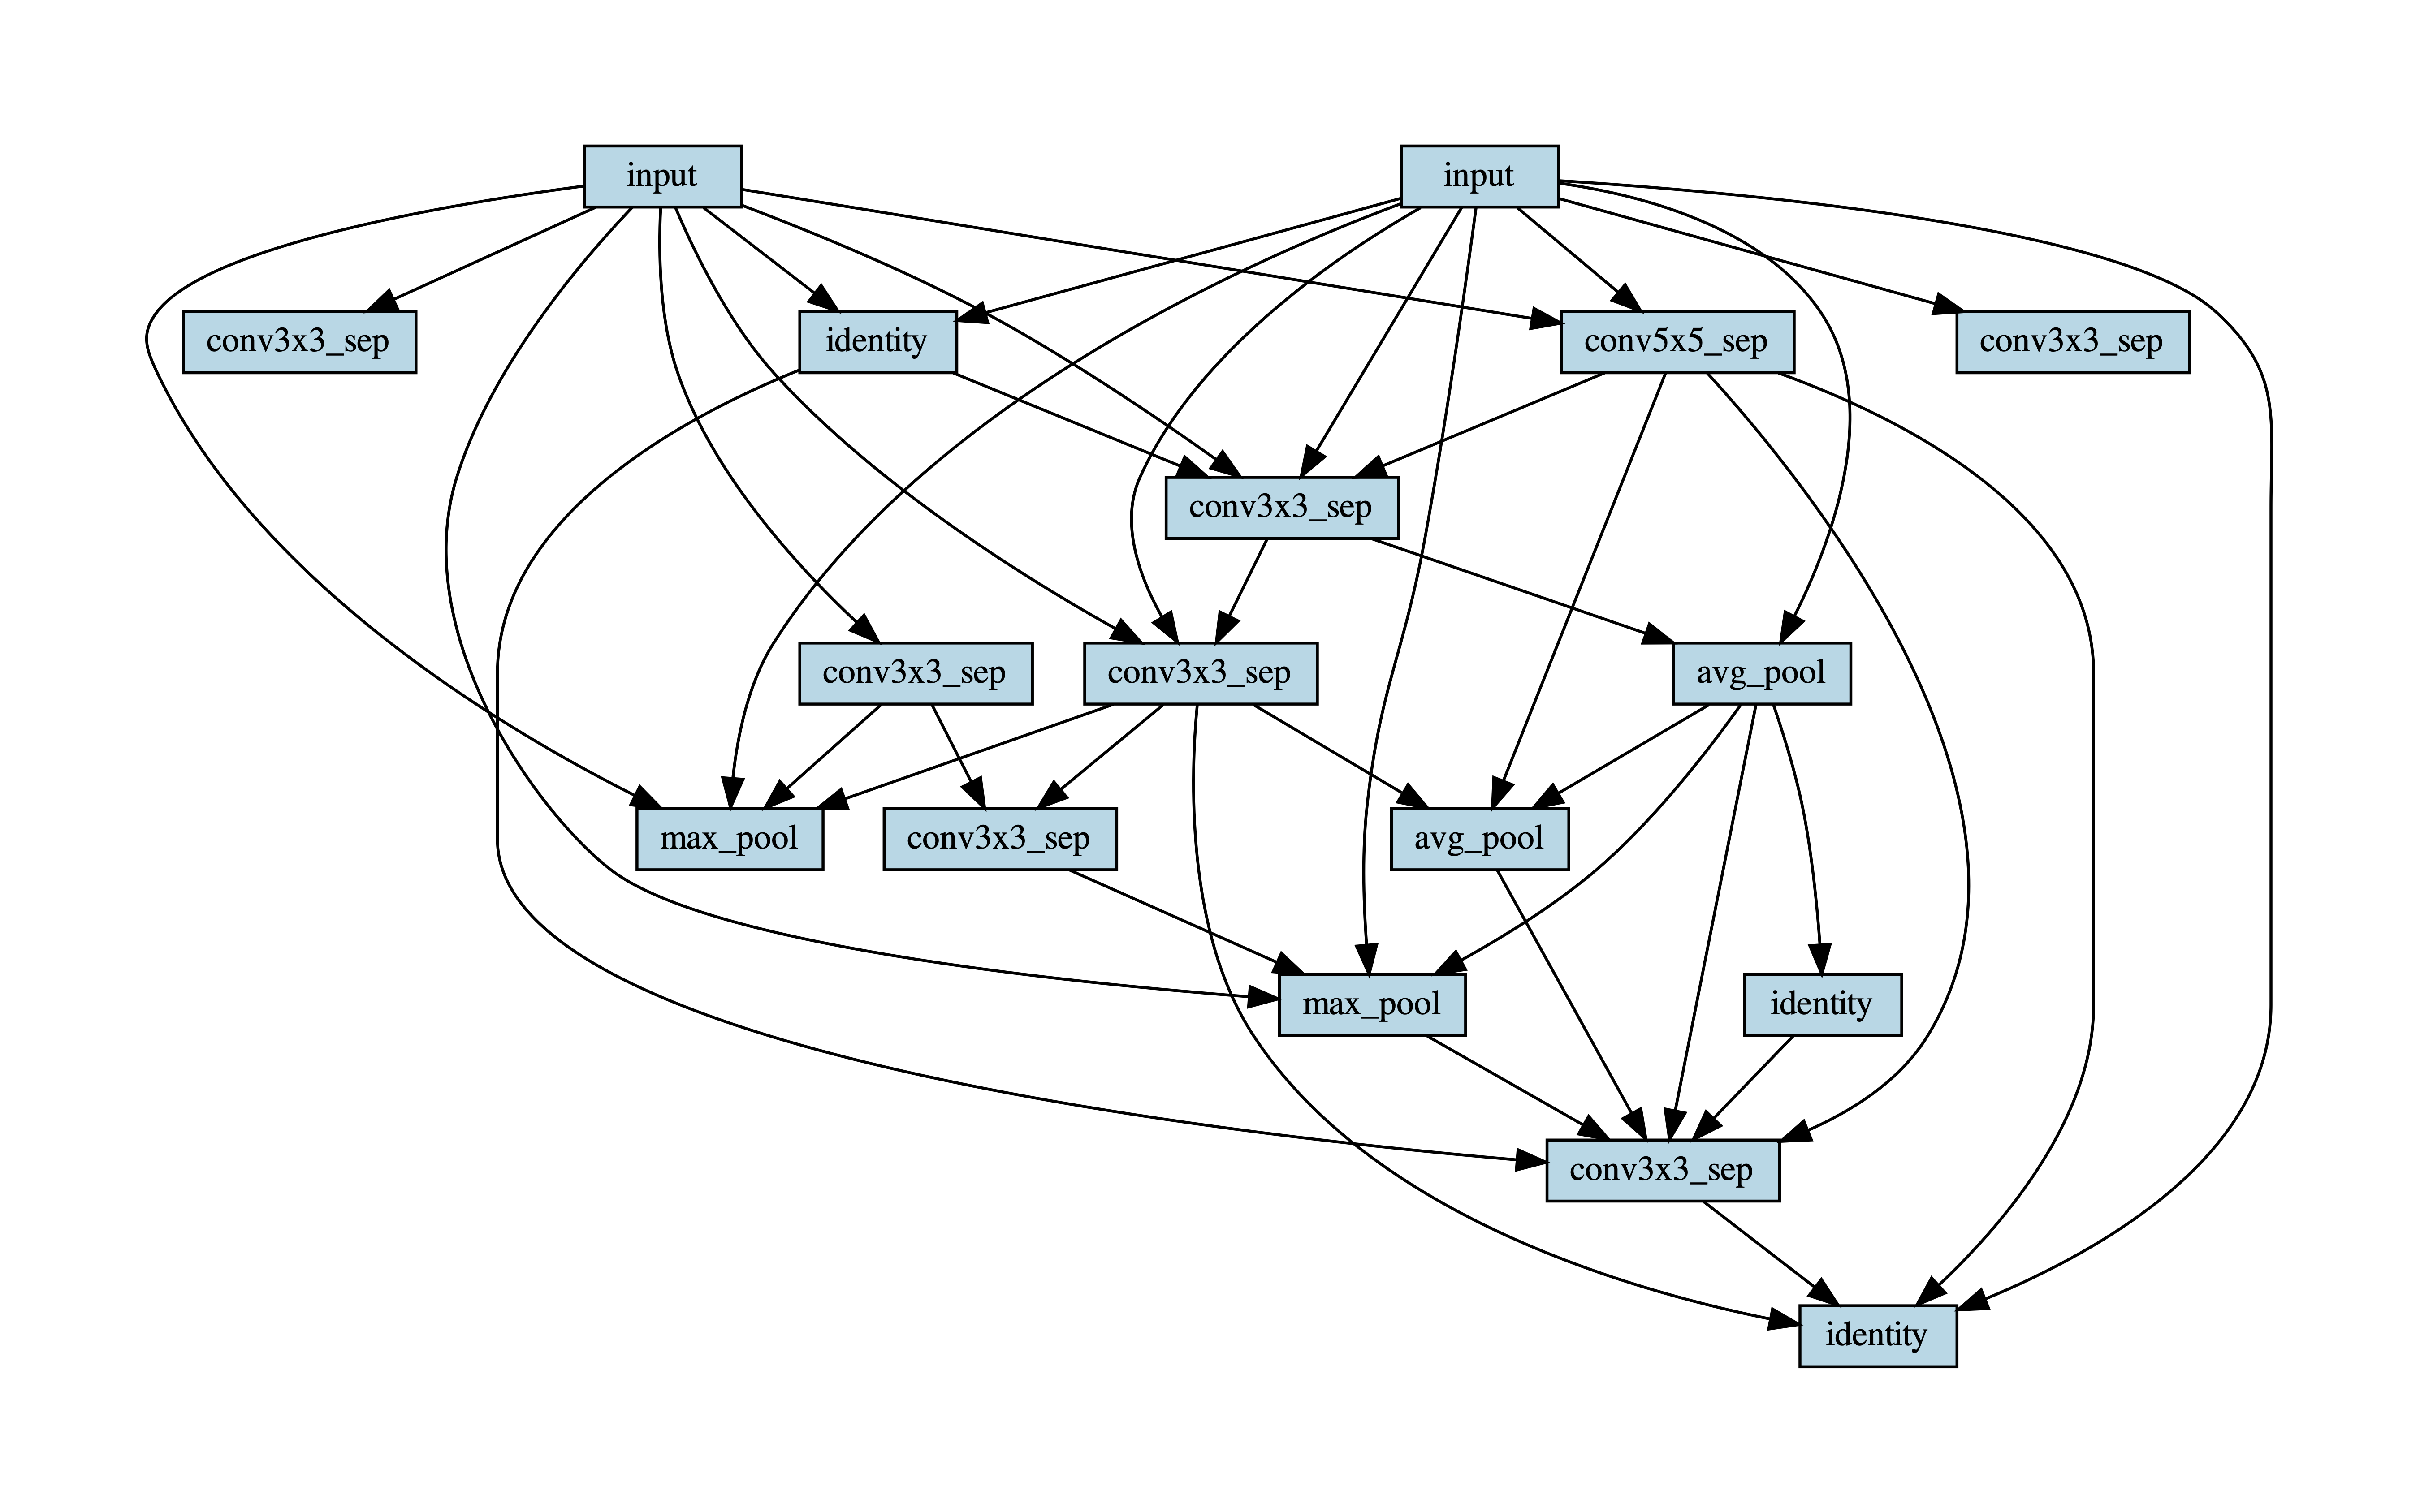
\includegraphics[width=6\linewidth]{figures/graph_-2132791772218152156.png}
\else
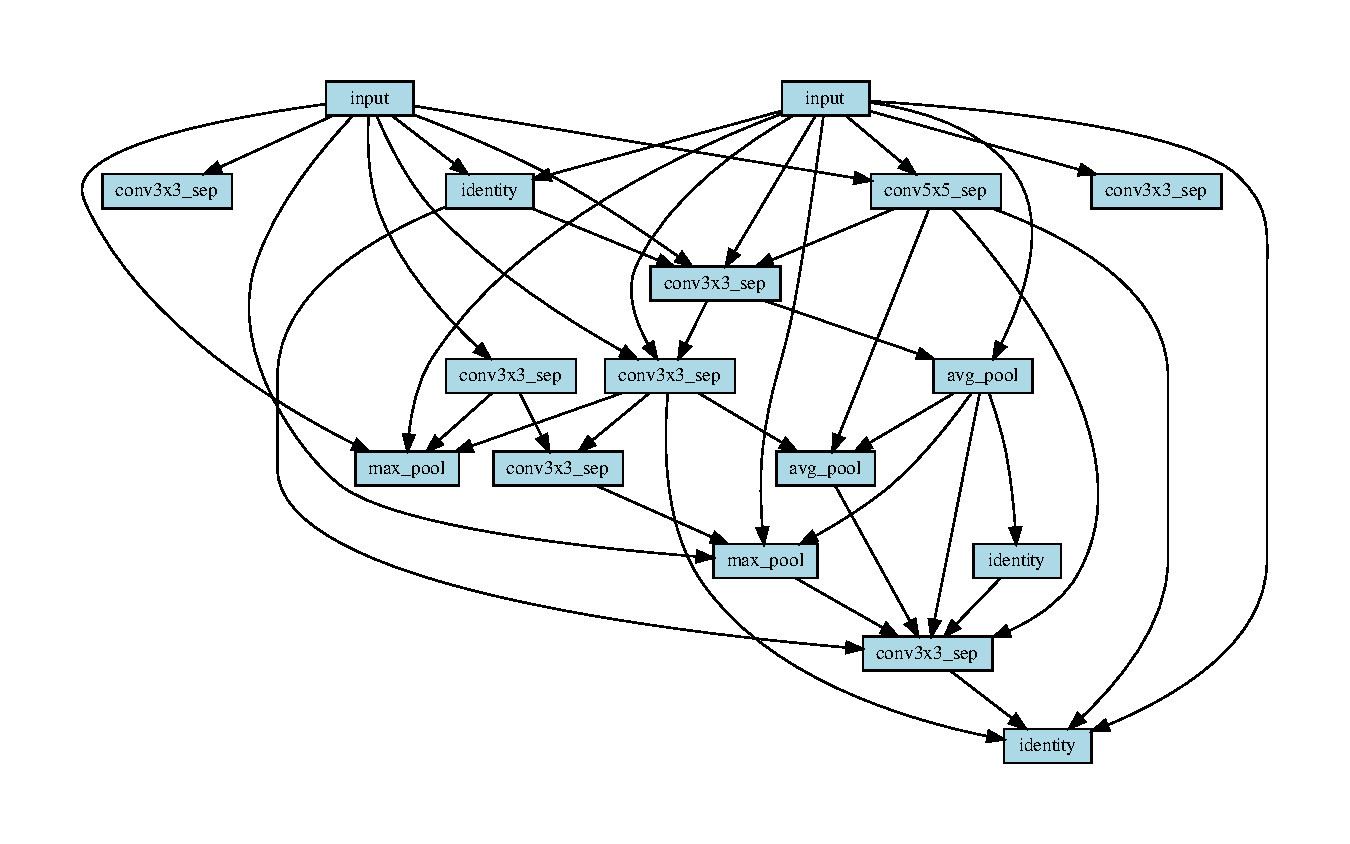
\includegraphics[width=\linewidth]{figures/graph_-2132791772218152156.pdf}
\fi
\caption{Best block found for classification}
\label{fig:best_block}
\end{figure}

\subsubsection{Anytime Prediction}
Figures \ref{fig:best_anytime1}, \ref{fig:best_anytime2} and \ref{fig:best_anytime3} show blocks 1 2 and 3 of the best architecture found in the anytime experiments. The color red denotes that an early exit is attached to the output of the node.

\begin{figure}[h]
\iflatexml
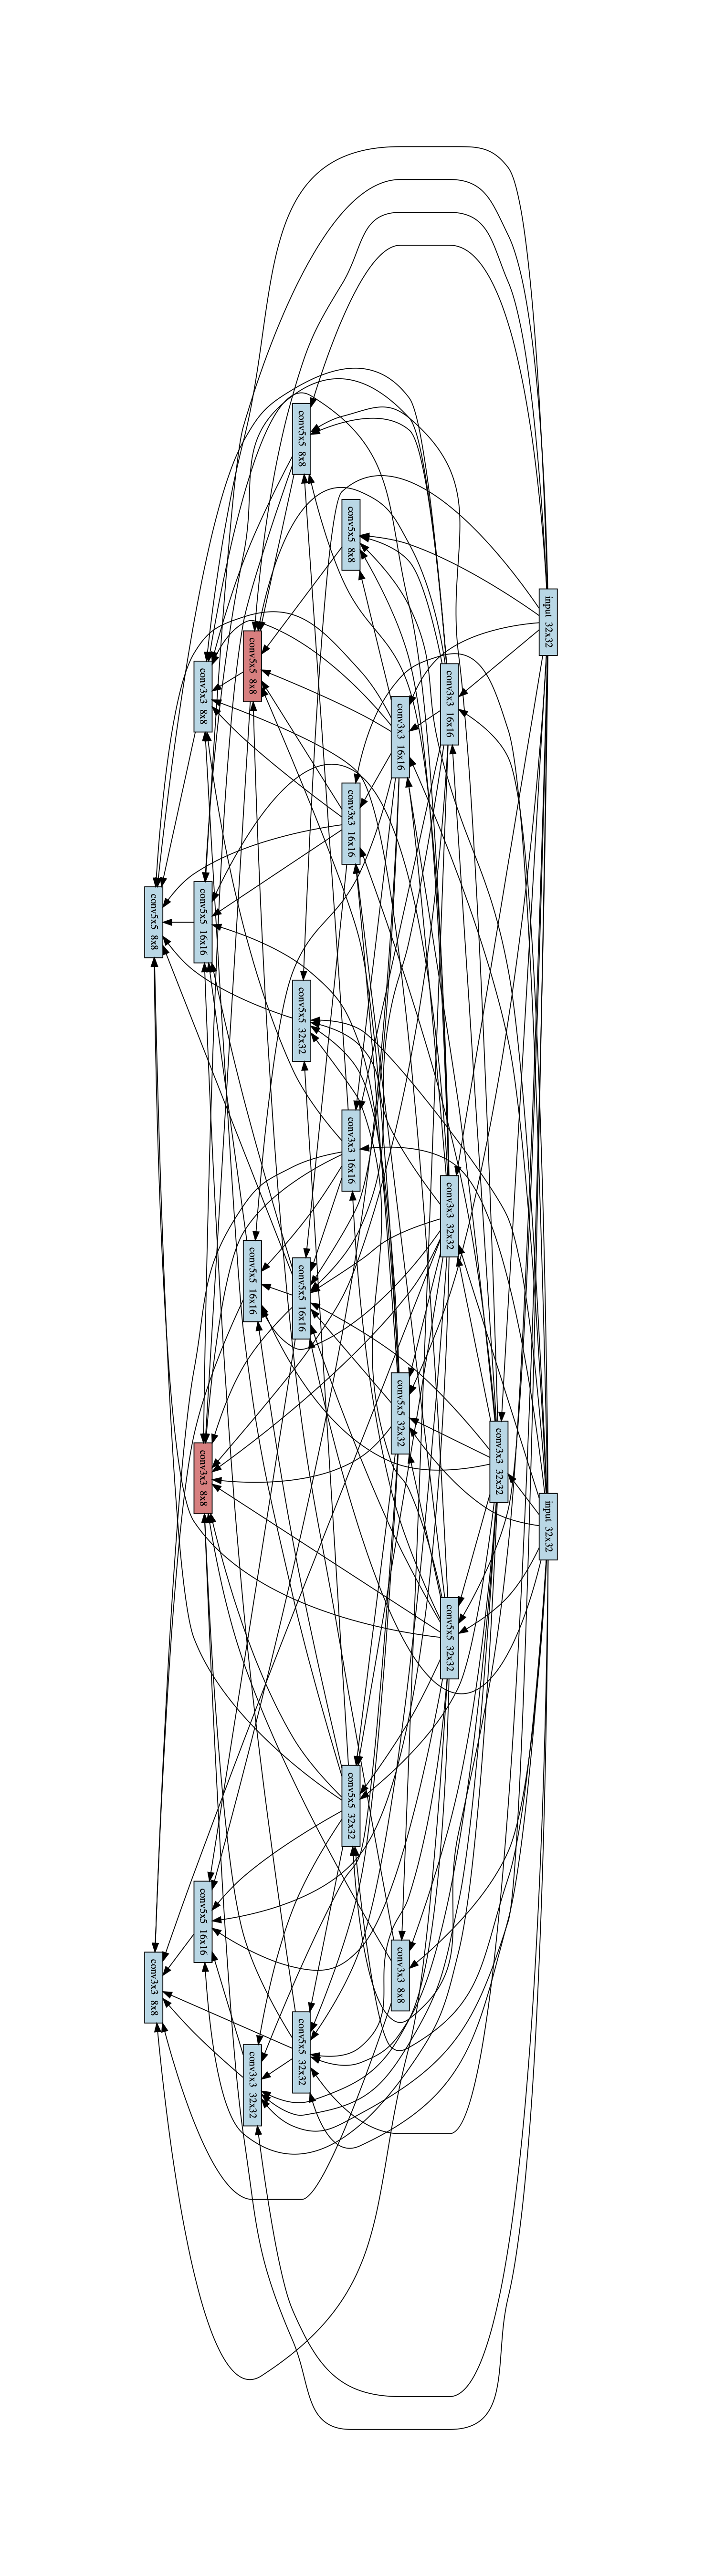
\includegraphics[width=6\linewidth]{figures/graph_642261663860860599_cell_0.png}
\else
\begin{center}
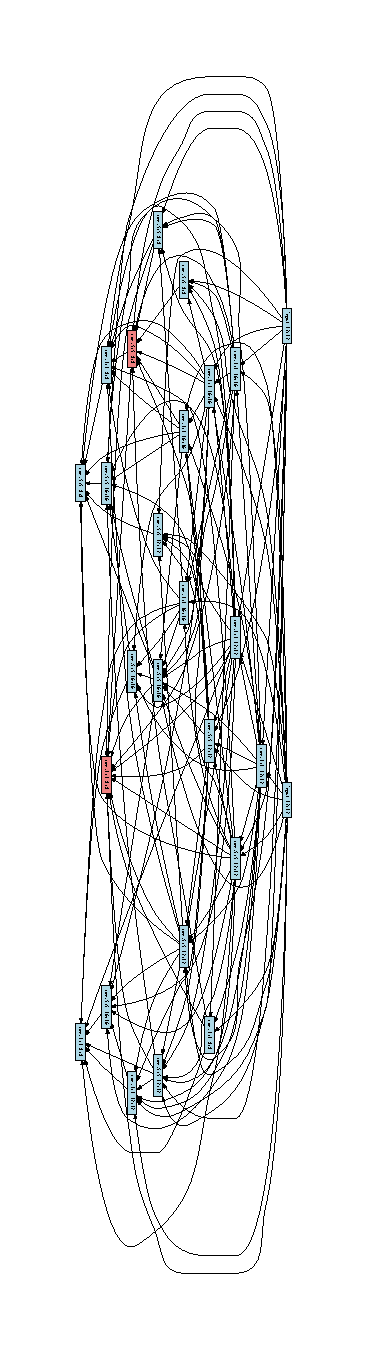
\includegraphics[width=0.4\linewidth]{figures/graph_642261663860860599_cell_0.pdf}
\end{center}
\fi
\caption{Block 1 for anytime network. Red color denotes early exit.}
\label{fig:best_anytime1}
\end{figure}


\begin{figure}[h]
\iflatexml
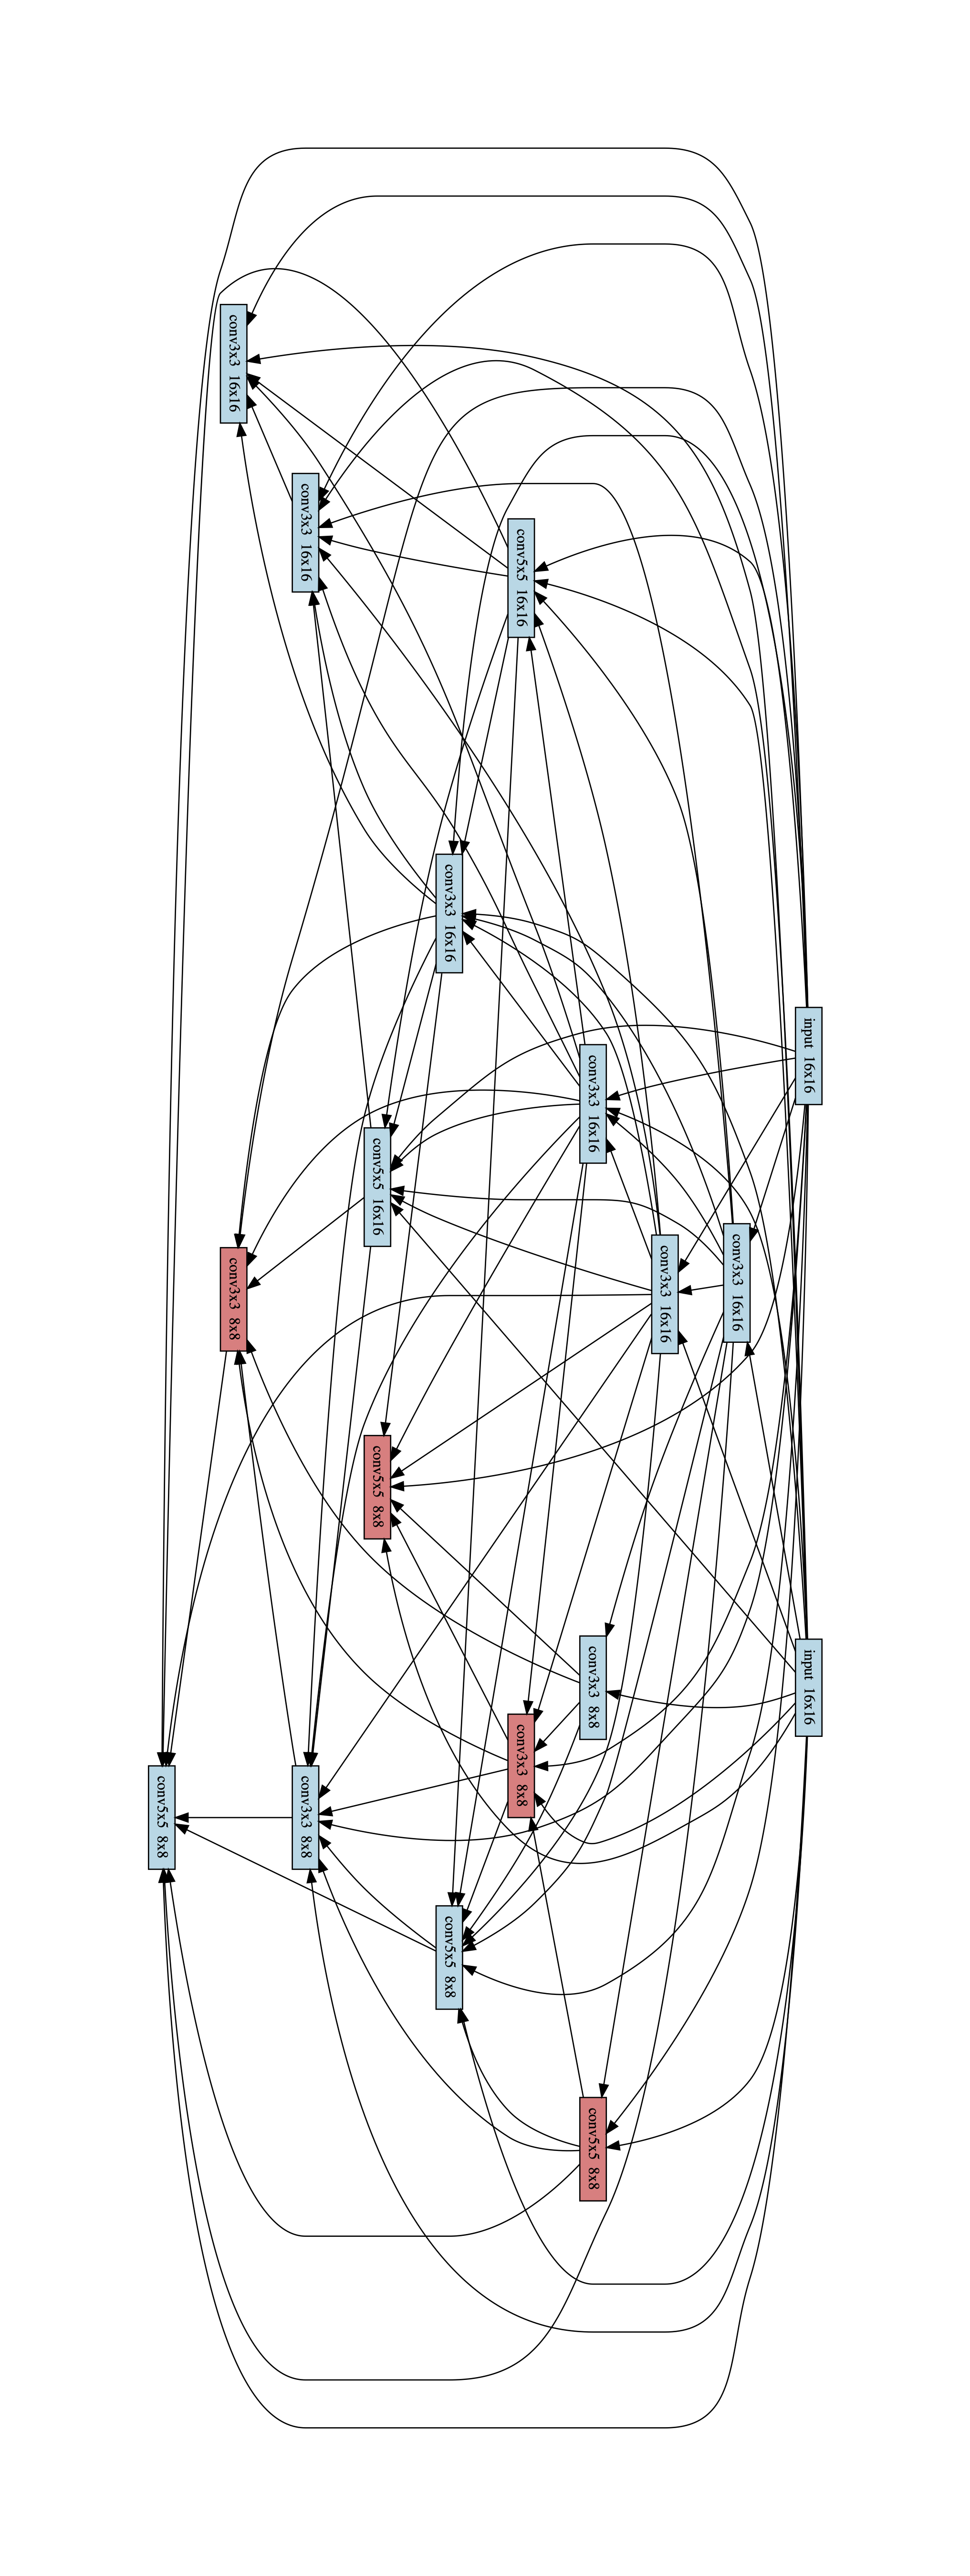
\includegraphics[width=6\linewidth]{figures/graph_642261663860860599_cell_1.png}
\else
\begin{center}
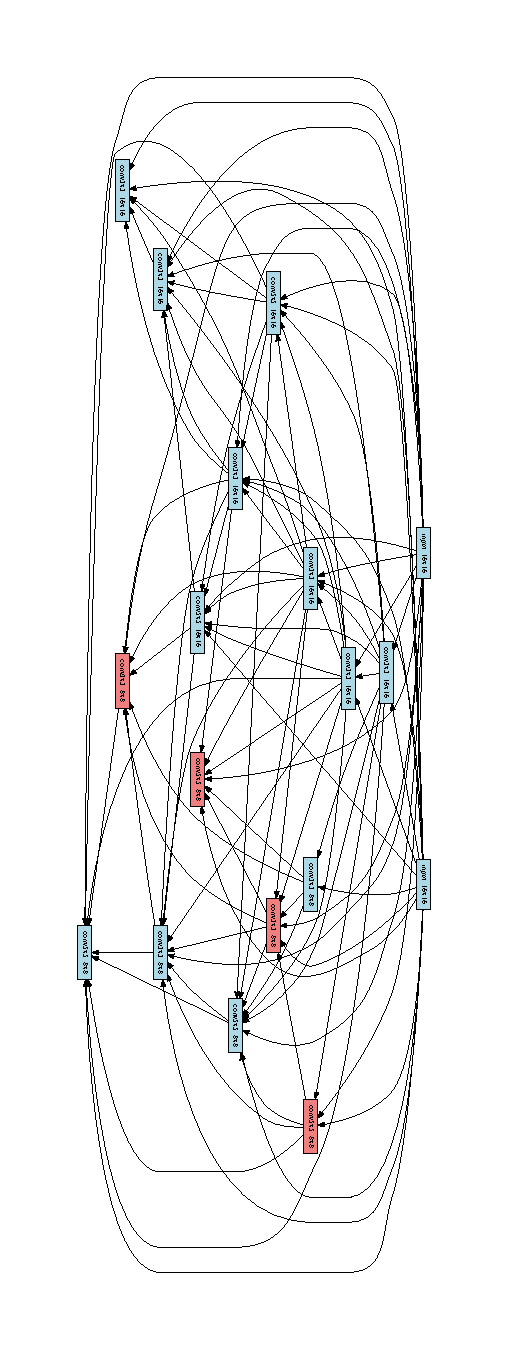
\includegraphics[width=0.6\linewidth]{figures/graph_642261663860860599_cell_1.pdf}
\end{center}
\fi
\caption{Block 2 for anytime network. Red color denotes early exit.}
\label{fig:best_anytime2}
\end{figure}


\begin{figure}[h]
\iflatexml
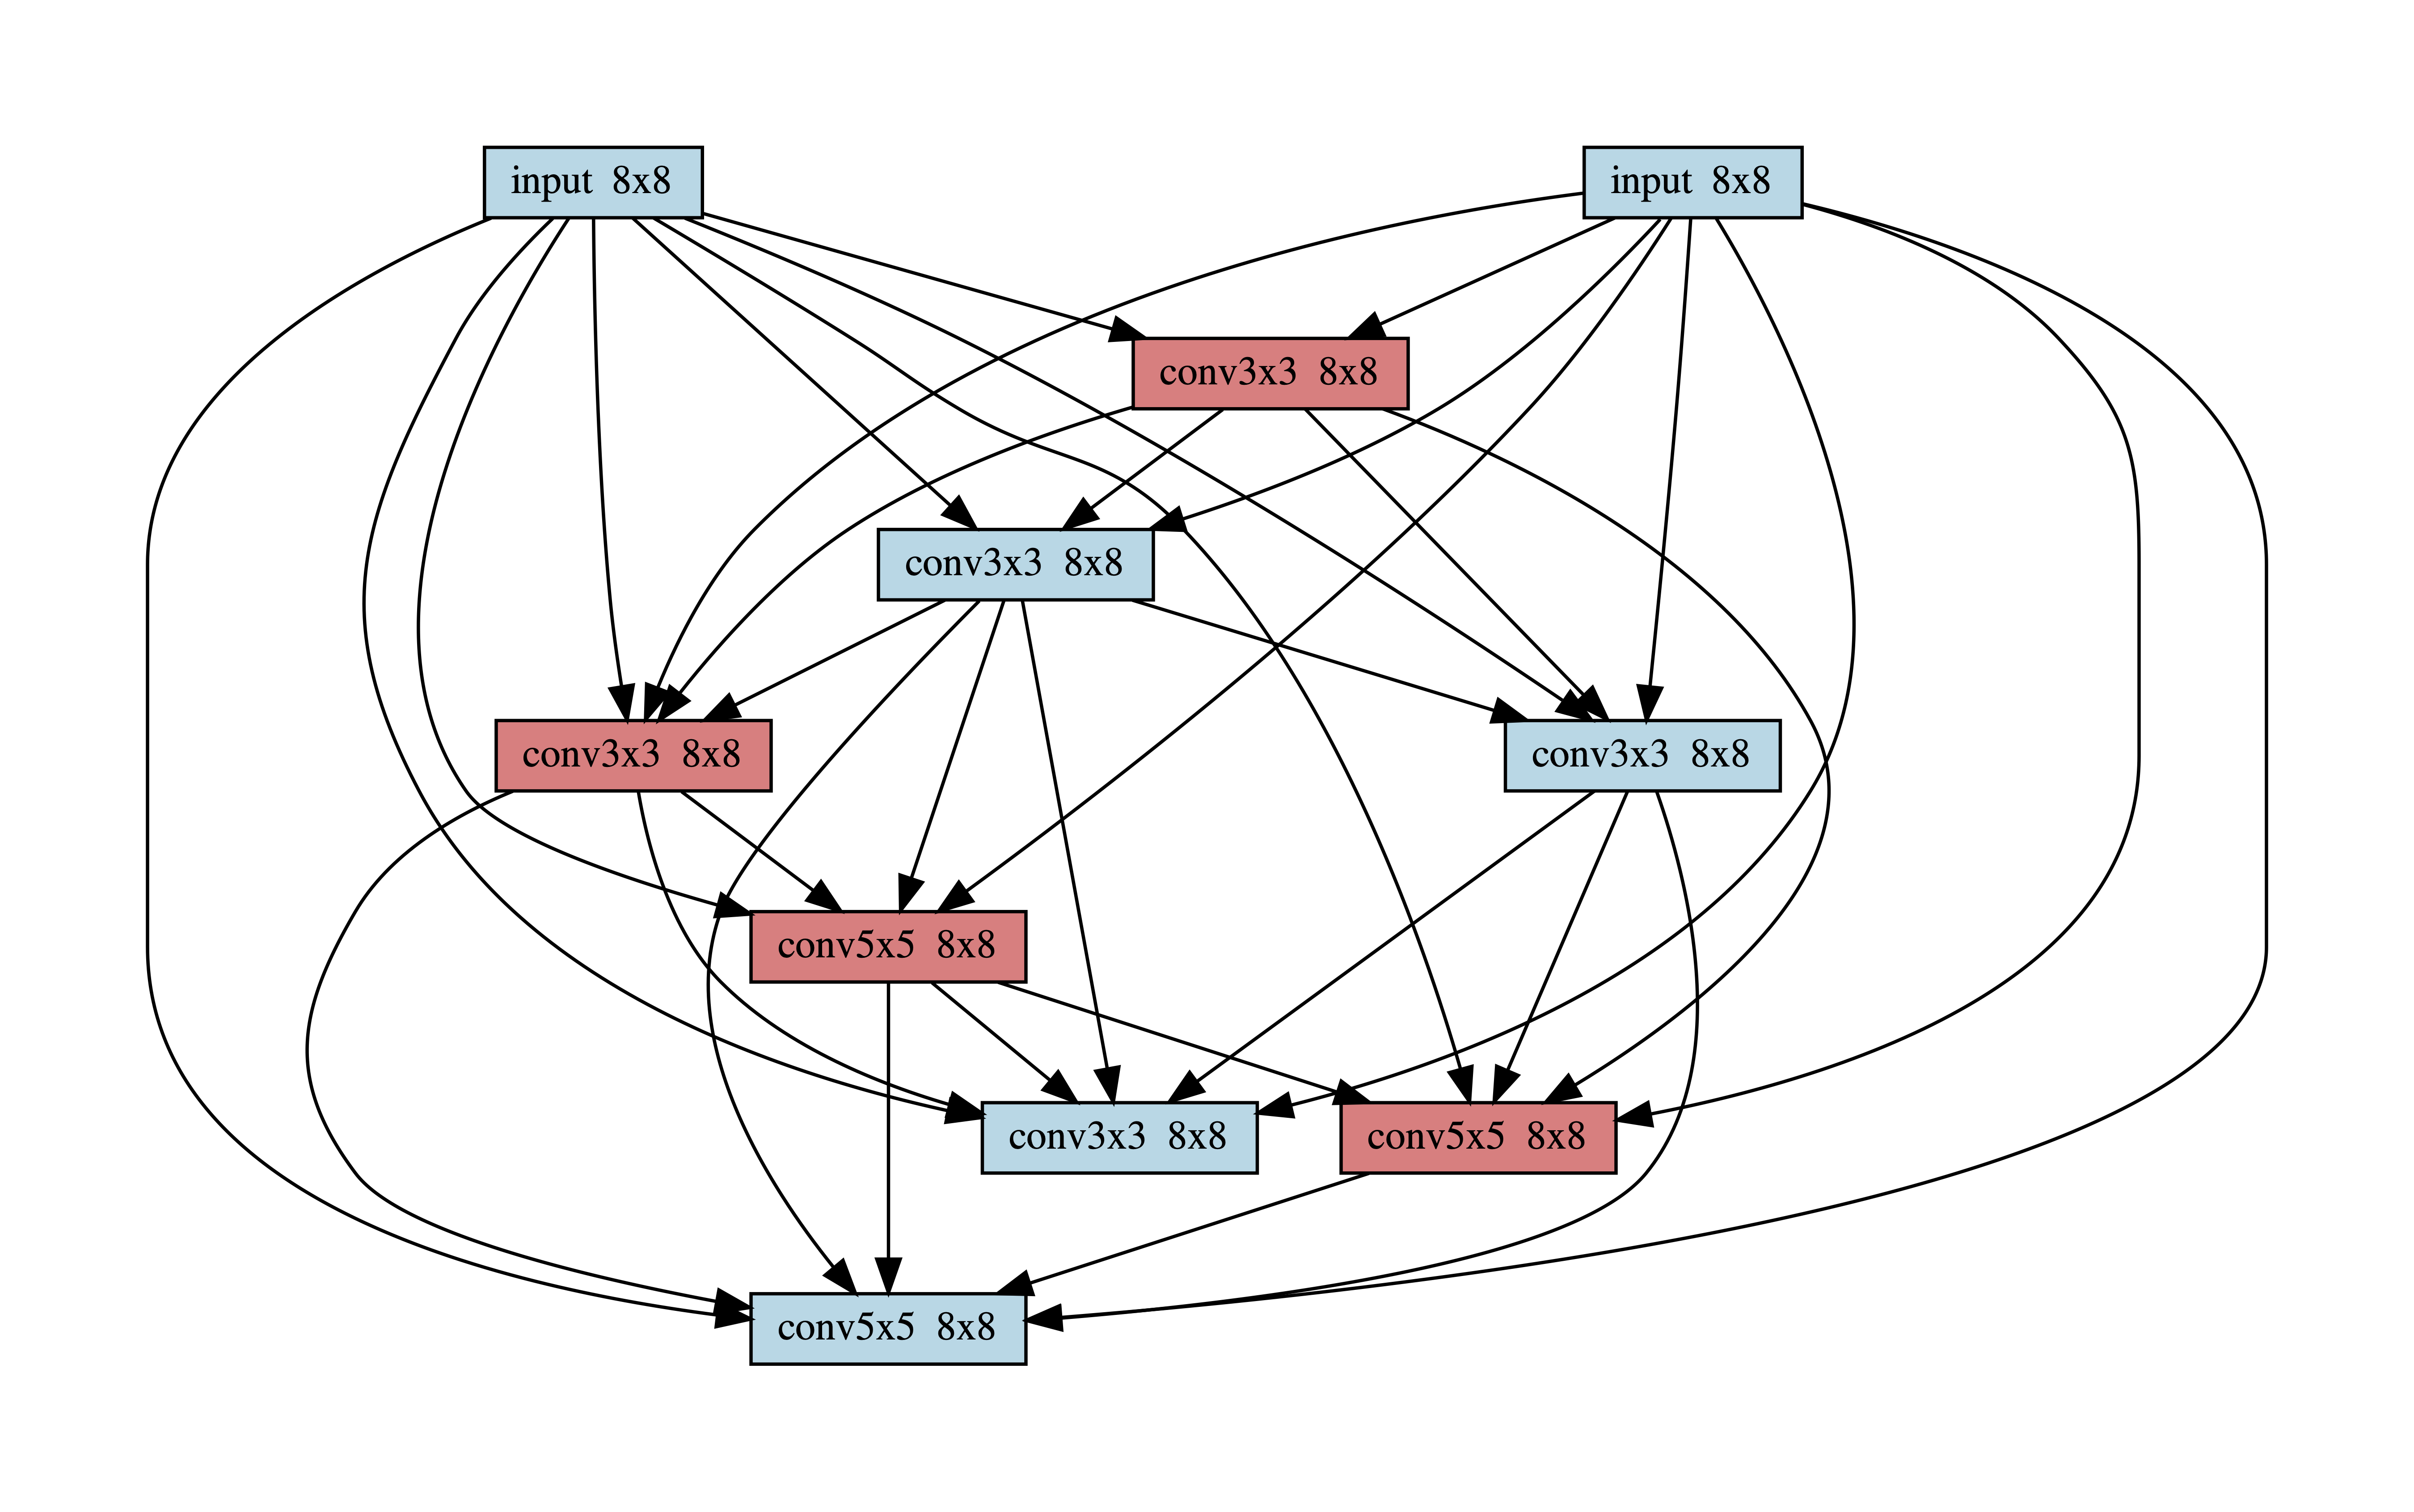
\includegraphics[width=6\linewidth]{figures/graph_642261663860860599_cell_2.png}
\else
\begin{center}
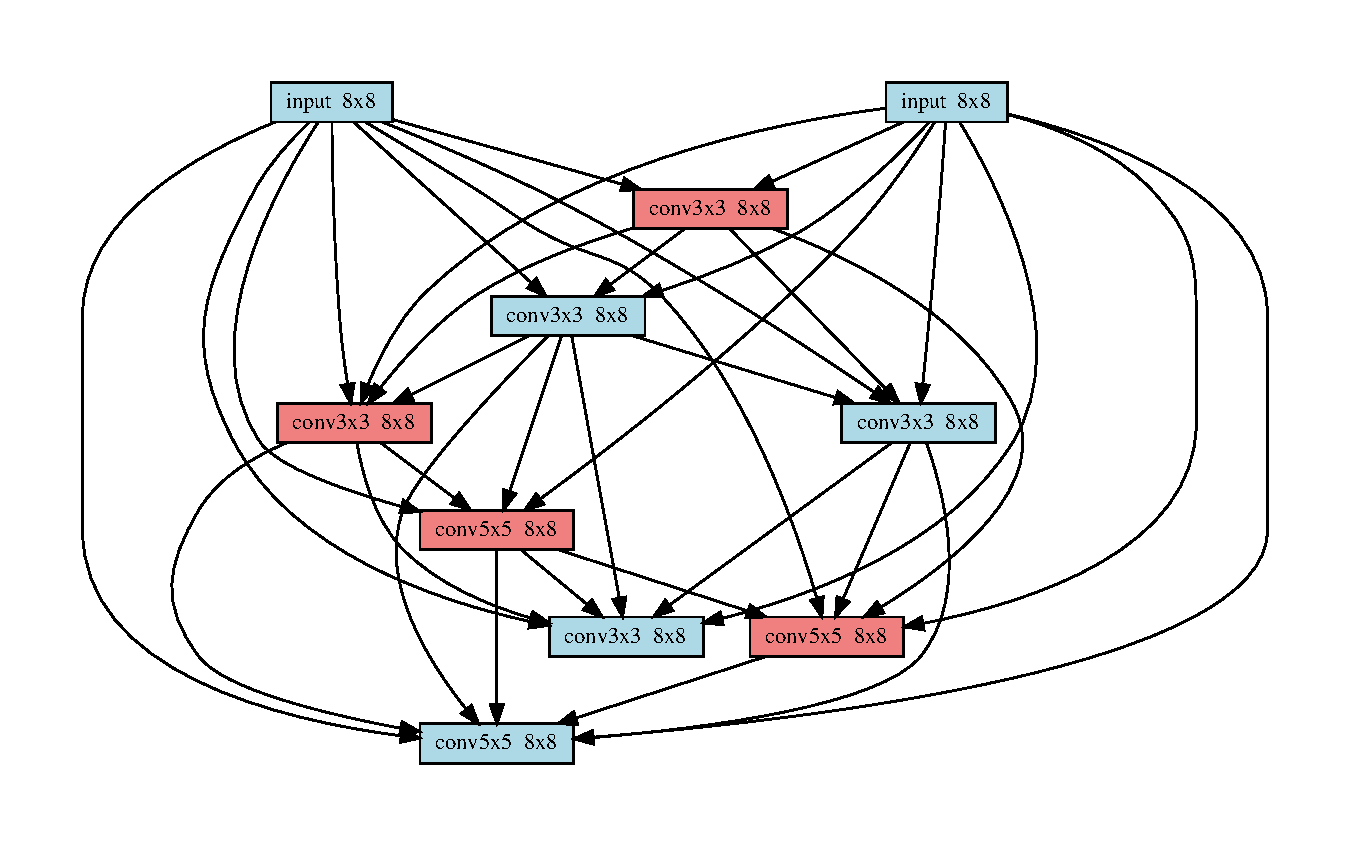
\includegraphics[width=\linewidth]{figures/graph_642261663860860599_cell_2.pdf}
\end{center}
\fi
\caption{Block 3 for anytime network. Red color denotes early exit.}
\label{fig:best_anytime3}
\end{figure}

%\subsection{GHN Settings}
%
%
%the recurrent cell function $U$ is  with latent dimension 32, 
%and the message function $M$ is a 2 layer MLP with a latent dimension of 32 and ReLU non-linearity. 


% Existin Nas methods \citep{zoph2017learning,real2018regularized} %